\documentclass[10pt, landscape]{extarticle}
\usepackage{ctex}
\usepackage{multicol}
\usepackage{calc}
\usepackage{ifthen}
\usepackage[landscape]{geometry}
\usepackage{hyperref}
\usepackage{lipsum}
\usepackage{amsmath}
\usepackage{graphicx}
\usepackage{float}
\usepackage{wrapfig}
\usepackage{xcolor}

\numberwithin{equation}{section}


% To make this come out properly in landscape mode, do one of the following
% 1.
%  pdflatex latexsheet.tex
%
% 2.
%  latex latexsheet.tex
%  dvips -P pdf  -t landscape latexsheet.dvi
%  ps2pdf latexsheet.ps


% If you're reading this, be prepared for confusion.  Making this was
% a learning experience for me, and it shows.  Much of the placement
% was hacked in; if you make it better, let me know...


% 2008-04
% Changed page margin code to use the geometry package. Also added code for
% conditional page margins, depending on paper size. Thanks to Uwe Ziegenhagen
% for the suggestions.

% 2006-08
% Made changes based on suggestions from Gene Cooperman. <gene at ccs.neu.edu>


% To Do:
% \listoffigures \listoftables
% \setcounter{secnumdepth}{0}


% This sets page margins to .5 inch if using letter paper, and to 1cm
% if using A4 paper. (This probably isn't strictly necessary.)
% If using another size paper, use default 1cm margins.
\ifthenelse{\lengthtest { \paperwidth = 11in}}
	{ \geometry{top=.2in,left=.2in,right=.2in,bottom=.2in} }
	{\ifthenelse{ \lengthtest{ \paperwidth = 297mm}}
		{\geometry{top=1cm,left=1cm,right=1cm,bottom=1cm} }
		{\geometry{top=1cm,left=1cm,right=1cm,bottom=1cm} }
	}

% Turn off header and footer
\pagestyle{empty}
 

% Redefine section commands to use less space
\makeatletter
\renewcommand{\section}{\@startsection{section}{1}{0mm}%
                                {-1ex plus -.5ex minus -.2ex}%
                                {0.5ex plus .2ex}%x
                                {\normalfont\large\bfseries}}
\renewcommand{\subsection}{\@startsection{subsection}{2}{0mm}%
                                {-1explus -.5ex minus -.2ex}%
                                {0.5ex plus .2ex}%
                                {\normalfont\normalsize\bfseries}}
\renewcommand{\subsubsection}{\@startsection{subsubsection}{3}{0mm}%
                                {-1ex plus -.5ex minus -.2ex}%
                                {1ex plus .2ex}%
                                {\normalfont\small\bfseries}}
\makeatother

% Define BibTeX command
\def\BibTeX{{\rm B\kern-.05em{\sc i\kern-.025em b}\kern-.08em
    T\kern-.1667em\lower.7ex\hbox{E}\kern-.125emX}}

% Don't print section numbers
% \setcounter{secnumdepth}{0}


\setlength{\parindent}{0pt}
\setlength{\parskip}{0pt plus 0.5ex}


\newcommand{\dd}{\mathrm{d}}
\newcommand{\pp}{\partial}


% -----------------------------------------------------------------------

\begin{document}

\raggedright
\footnotesize
\begin{multicols}{3}
\section{导论}
\section{燃烧与热化学}
\subsection{概述}
\subsection{热力学参数关系式回顾}
\subsubsection{广延量和强度量}
\textbf{广延量:}取决于物质的数量(质量或物质的量),一般大写;{\textbf{强度量:}单位质量(或物质的量)来表示},数值与物质的量无关。\textit{单位物质的量的在本书中会加上划线},如$\overline{u}$,单位质量的则不加划线,如$u$。

\subsubsection{状态方程}
\begin{eqnarray}
    PV&=&nR_uT\\
    PV&=&mRT\\
    Pv&=&RT\\
    P&=&\rho RT
\end{eqnarray}
$R_u=8315~\mathrm{J/(kmol\cdot K)}$, $R=R_u/\mathrm{MW}$, $\rho=1/v=m/V$.

\subsubsection{状态热方程}
\begin{eqnarray}
    u&=&u(T,v)\\
    h&=&h(T, P)
\end{eqnarray}
\begin{eqnarray}
    \mathrm{d}u&=&\left({\frac{\partial u}{\partial T}}\right)_{v}\mathrm{d}T+\left({\frac{\partial u}{\partial v}}\right)_{T}\mathrm{d}v\\ 
    \mathrm{d}h&=&\left({\frac{\partial h}{\partial T}}\right)_{p}\mathrm{d}T+\left({\frac{\partial h}{\partial P}}\right)_{T}\mathrm{d}P
\end{eqnarray}
\begin{eqnarray}
    c_{v}&\equiv&\left(\frac{\partial u}{\partial T}\right)_{v}\\
c_{p}&\equiv&\left({\frac{\partial h}{\partial T}}\right)_{P}
\end{eqnarray}

对于理想气体,$(\partial u/\partial v)_T$和$(\partial h/\partial P)_{T}$都为0。所以理想气体的状态热方程为:
\begin{eqnarray}
    u(T)-u_{\mathrm{ref}}&=&\int_{T_{\mathrm{ref}}}^{T}c_{v}\,\mathrm{d}T\\ 
    h(T)-h_{\mathrm{ref}}&=&\int_{T_{\mathrm{ref}}}^{T}c_{p}\,\mathrm{d}T.
\end{eqnarray}

\subsubsection{理想气体混合物}
组份$i$的摩尔分数$\chi_i$:
\begin{equation}
    \chi_{i}\equiv\frac{N_{i}}{N_{1}+N_{2}+\cdots+N_{i}+\cdots}=\frac{N_{i}}{N_{\mathrm{tot}}}
\end{equation}
组份$i$的质量分数$Y_i$:
\begin{equation}
    Y_{i}\equiv\frac{m_{i}}{m_{1}+m_{2}+\cdots+m_{i}+\cdots}=\frac{m_{i}}{m_{\mathrm{tot}}}
\end{equation}
他们之间存在着如下的换算关系:
\begin{equation}
    Y_{i}=\chi_{i}\mathrm{M}\mathrm{W}_{i}/\mathrm{M}\mathrm{W}_{\mathrm{mix}}
\end{equation}
\begin{equation}
    \chi_{i}=Y_{i}\mathrm{MW}_{\mathrm{mix}}/\mathrm{MW}
\end{equation}
对于混合物的摩尔质量:
\begin{equation}
    \mathrm{MW}_\mathrm{mix} = \sum_i \chi_i \mathrm{MW}_i
\end{equation}
\begin{equation}
    \mathrm{MW}_\mathrm{mix} = \frac{1}{\sum_i (Y_i/\mathrm{MW}_i)}
\end{equation}

混合物的强度量可以用各物质的强度量加权计算得到,对于组份的熵,我们有:
\begin{equation}
    s_{i}(T,P_{i})=s_{i}(T,P_{\mathrm{ref}})-R\ln{\frac{P_{i}}{P_{\mathrm{ref}}}}
\end{equation}
\begin{equation}
    \bar{s}_{i}(T,P)=\bar{s}_{i}(T,P_{\mathrm{ref}})-R_{u}\ln{\frac{P_{i}}{P_{\mathrm{ref}}}}\,.
\end{equation}

\subsubsection{蒸发潜热}
aka 蒸发焓,
\begin{equation}
    h_{fg}(T,P)\equiv h_{\mathrm{vapor}}(T,P)-h_{\mathrm{liquid}}(T,P),
\end{equation}

给定温度和压力计算蒸发潜热的方法,Clausius-Claperon方程,
\begin{equation}
    \frac{\mathrm{d}P_{\mathrm{sat}}}{P_{\mathrm{sat}}}=\frac{h_{f g}}{R}\,\frac{\mathrm{d}T_{\mathrm{sat}}}{T_{\mathrm{sat}}^{2}}.
\end{equation}

\subsection{热力学第一定律}
\subsubsection{第一定律——定质量}
\subsubsection{第一定律——控制体}

\subsection{反应物和生成物的混合物}
\subsubsection{化学计量学}
对于碳氢燃料C$_x$H$_y$,
\begin{equation}
    \begin{aligned}
        &C_x\mathrm{H}_y + a(\mathrm{O}_2 + 3.76\mathrm{N}_2)\rightarrow\\
        & x\mathrm{CO}_2 + \frac{y}{2}\mathrm{H}_2\mathrm{O} + 3.76a\mathrm{N}_2
    \end{aligned}
\end{equation}



其中,
$$
a=x+y/4.
$$
\textbf{化学当量的空-燃比}:
\begin{equation}
    (A/F)_{\mathrm{stolc}}=\left(\frac{m_{\mathrm{air}}}{m_{\mathrm{fuel}}}\right)_{\mathrm{stoic}}=\frac{4.76a}{1}\frac{M W_{\mathrm{air}}}{MW_{\mathrm{fuel}}},
\end{equation}
\textbf{当量比}:
\begin{equation}
    \Phi={\frac{(A/F)_{\mathrm{stoic}}}{(A/F)}}={\frac{(F/A)}{(F/A)_{\mathrm{stoic}}}}
\end{equation}
当量空气百分比=100\%/$\Phi$,过量空气百分比=(1-$\Phi$)/$\Phi\times$100\%

\subsubsection{绝对(或标准)焓和生成焓}

绝对焓=标准生成焓+显焓的变化,

\begin{equation}
    \overline{h}_i(T) = \overline{h}_{f,i}^0(T_\mathrm{ref})+\Delta\overline{h}_{s,i}(T),
\end{equation}

\textbf{参考温度:}$T_\mathrm{ref}=25^\circ \mathrm{C}$(298.15 K),\textbf{参考压力:}$P_\mathrm{ref}=$1atm(101 325 Pa)。

对于标准生成焓:元素最自然状态时的生成焓为0,比如氧气,氮气等。

\subsubsection{燃烧焓和热值}
\textbf{燃烧焓}定义为(反应物和产物\textit{都处于标准状态下}):
\begin{equation}
    \Delta h_{R}\equiv q_{c v}=h_{\mathrm{prod}}-h_{\mathrm{reac}},
\end{equation}
\textbf{燃烧热}$\Delta h_c$(也称为热值)为燃烧焓的相反数。
\begin{itemize}
    \item \textbf{高位热值}(HHV):假设所有的产物都凝结成液化水时的燃烧热。
    \item \textbf{地位热值}(LHV):没有水凝结成液态的情况下的燃烧热。
\end{itemize}

\subsection{绝热燃烧温度}

\textbf{定压绝热燃烧温度: }
\begin{equation}
    h_{\mathrm{reac}}(T_{i},P)=h_{\mathrm{prod}}(T_{a d},P).
\end{equation}

\begin{figure}[H]
    \centering
    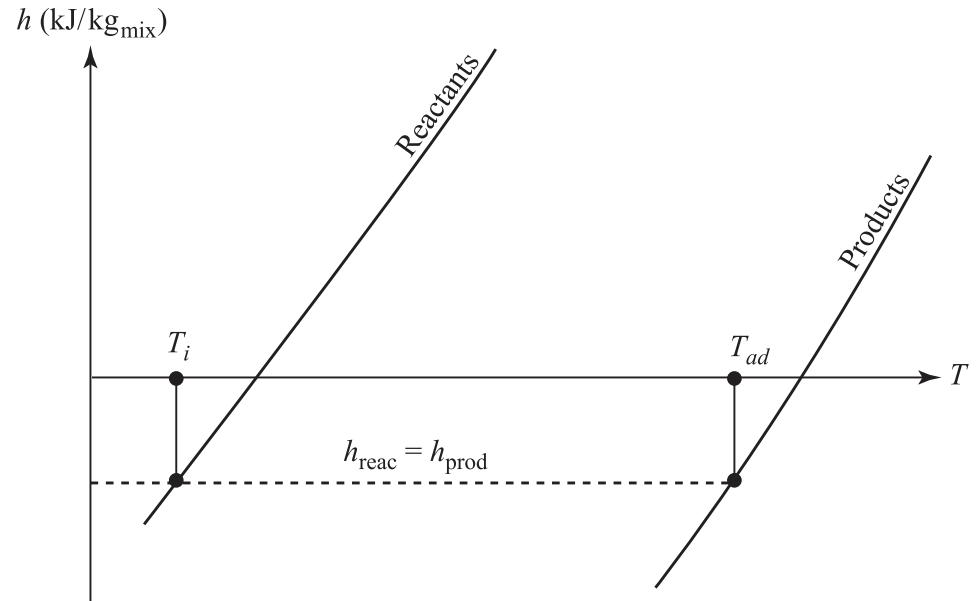
\includegraphics[width=.23\textwidth]{img/ad_T.png}
\end{figure}

\textbf{定容绝热燃烧温度:}反应前后内能相等,
\begin{equation}
    U_{\mathrm{reac}}(T_{\mathrm{init}},P_{\mathrm{init}})=U_{\mathrm{prod}}(T_{a d},P_{f}),
\end{equation}

写成焓的形式:
\begin{equation}
    \begin{aligned}
        H_{\mathrm{reac}}-H_{\mathrm{prod}}-V(P_{\mathrm{init}}-P_{f})&=0.\\
        H_{\mathrm{reac}}-H_{\mathrm{prod}}-R_{u}(N_{\mathrm{reac}}T_{\mathrm{init}}-N_{\mathrm{prod}}T_{a d})&=0.
    \end{aligned}
\end{equation}

\subsection{化学平衡}
\subsubsection{第二定律的讨论}

单个组份的熵计算公式:
\begin{equation}
    \overline{{{s}}}_{i}=\overline{{{s}}}_{i}^{0}(T_{\mathrm{ref}})+\int_{T_{\mathrm{ef}}}^{T_{f}}\overline{{{c}}}_{p,i}\,\frac{\mathrm{d}T}{T}-R_{u}\,\ln\frac{P_{i}}{P^{0}},
\end{equation}

对于封闭系统,反应自发发生的条件为$\mathrm{d}S\ge 0$。平衡条件为:$(\mathrm{d}S)_{U,V,m}=0$。

\subsubsection{吉布斯函数}

单个组份的吉布斯函数的计算:

\begin{equation}
    \overline{{{g}}}_{i,T}=\overline{{{g}}}_{i,T}^{o}+R_{u}T\ln\left(P_{i}/P^{o}\right)
\end{equation}

对于开口系统,我们采用吉布斯函数,它的定义为 $G\equiv H-TS$。这是第二定律表示为$(\mathrm{d}G)_{T,P,m}\le 0$的形式。在平衡时,开口系统的第二定律可以写作$(\mathrm{d}G)_{T,P,m}=0$。

{
    \scriptsize\color{gray}
    考虑广延量,理想气体的吉布斯方程为:
    \[
        G_{\mathrm{mix}}=\sum N_{i}\overline{{{g}}}_{i,T}=\sum N_{i}\bigl[\bar{g}_{i,T}^{0}+R_{u}T\ln\bigl(P_{i}/P^{0}\bigr)\bigr]
    \]
    对上面的式子取微分,得到平衡条件,可以写作:
    \[
        \begin{aligned}
        &\sum{\mathrm{d}{N}}_{i}\left[\bar{g}_{i,T}^{0}+R_{u}T\ln\left(P_{i}/P^{0}\right)\right]+\\
        &\sum{N}_{i}\mathrm{d}\left[\bar{g}_{i,T}^{0}+R_{u}T\ln\left(P_{i}/P^{0}\right)\right]=0.
        \end{aligned}
    \]
    考虑到总压不变,也就是分压变化的和不变,因此式子中的第二项等于零,它可以被简化为:
    \[\sum{\mathrm{d}{N}}_{i}\left[\bar{g}_{i,T}^{o}+R_{u}T\ln\left(P_{i}/P^{0}\right)\right]=0\]
    对于一个一般的系统,我们将化学反应写作
    \[a\mathbf{A}+b\mathbf{B}+\cdots\leftrightarrow e\mathbf{E}+f\mathbf{F}+\cdots\]
    由于物质的摩尔数变化和化学计量数成正比,因此我们可以将平衡表达式展开写作:
    \[
        \begin{aligned}
            &-a\Bigl[\bar{g}_\mathrm{A,T}^{o}+R_{u}T\ln\bigl(P_{\mathrm{A}}/P^{o}\bigr)\Bigr]\\
            &-b\Bigl[\bar{g}_{\mathrm{B,T}}^{o}+R_{u}T\ln\bigl(P_{\mathrm{B}}/P^{o}\bigr)\Bigr]-\cdots\\
            &+e\Bigl[\overline{{{g}}}_{\scriptscriptstyle\mathrm{E,}T}^{o}+R_{u}T\ln\bigl(P_{\scriptscriptstyle\mathrm{E}}/P^{o}\bigr)\Bigr]\\
            &+f\Bigl[\overline{{{g}}}_{\scriptscriptstyle\mathrm{F,}T}^{o}+R_{u}T\ln\bigl(P_{\scriptscriptstyle\mathrm{F}}/P^{o}\bigr)\Bigr]+\cdots=0.
        \end{aligned}
    \]
    合并整理一下不难得到:
    \[
        \begin{aligned}
            &-\Bigl(e\bar{g}_{\mathrm{E},T}^{o}+f\overline{{{g}}}_{\mathrm{F},T}^{o}+\cdot\cdot\cdot-a\overline{{{g}}}_{\mathrm{A},T}^{o}-b\overline{{{g}}}_{\mathrm{B},T}^{o}-\cdots\Bigr)\\
            &=R_{u}T\ln{\frac{\left(P_{\mathrm{E}}/P^{o}\right)^{e}\cdot\left(P_{\mathrm{F}}/P^{o}\right)^{f}\cdot\mathrm{etc.}}{\left(P_{\mathrm{A}}/P^{o}\right)^{a}\cdot\left(P_{\mathrm{B}}/P^{o}\right)^{b}\cdot\mathrm{etc.}}}
        \end{aligned}\]
}
我们定义\textbf{标准状态吉布斯函数差 $\Delta G_T^0$}为:
\begin{equation}
    \Delta G_T^0 = (e\bar{g}_{\mathrm{E},T}^{o}+f\overline{{{g}}}_{\mathrm{F},T}^{o}+\cdot\cdot\cdot-a\overline{{{g}}}_{\mathrm{A},T}^{o}-b\overline{{{g}}}_{\mathrm{B},T}^{o}-\cdots)
\end{equation}
\textbf{平衡常数 \(K_p\)}为:
\begin{equation}
    K_{p}={\frac{\left(P_{\mathrm{E}}/P^{o}\right)^{e}\cdot\left(P_{\mathrm{F}}/P^{o}\right)^{f}\cdot\mathrm{etc.}}{\left(P_{\mathrm{A}}/P^{o}\right)^{a}\cdot\left(P_{\mathrm{B}}/P^{o}\right)^{b}\cdot\mathrm{etc.}}}.
\end{equation}
这时,定压,定温条件下的化学平衡表达式就可以被写作:
\begin{equation}
    \Delta G_T^0 = -R_u T\ln K_p
\end{equation}
\begin{itemize}
    \item 如果\(\Delta G_T^0\)大于零,那么\(K_p\)小于1,反应向左进行(偏向反应物、几乎不反应)。
    \item 如果\(\Delta G_T^0\)小于零,那么\(K_p\)大于1,反应向右进行(偏向产物,趋于完全反应)。
\end{itemize}

{
    \scriptsize
    如果将\(\Delta G_T^0\)写作:
    \[
        \Delta G_T^0 = \Delta H^0 - T\Delta S^0
    \]
    的形式,平衡常数可以被写作:
    \[
        K_p = \mathrm{e}^{-\Delta H^0/R_u T}\cdot \mathrm{e}^{\Delta S^0/R_u}
    \]
    不难发现,
    \begin{itemize}
        \item 当反应的焓变小于零,反应放热,系统能量降低;
        \item 熵变大于零。
    \end{itemize}都会导致反应偏向于产物,\(K_p>1\)。
}

\subsubsection{复杂系统}

\subsection{燃烧的平衡产物}
\subsubsection{全平衡}
考虑实际的燃烧过程,最大燃烧温度一般发生在略微富燃料当量比的状态(\(\Phi\approx 1.05)\)。

\section{传质引论}
\subsection{概述}
\subsection{传质入门}
\subsubsection{传质速率定律}
\begin{itemize}
    \item 菲克扩散定律
    对于一维双组份扩散的情况:
    \begin{equation}\label{equ:fick_law_1d}
        \dot{m}_A'' = Y_A(\dot{m}_A'' + \dot{m}_B'') - \rho \mathcal{D}_\mathrm{AB}\frac{\dd Y_A}{\dd x}
    \end{equation}{\tiny 这里要特别注意,虽然\(\dot{m}_A'' + \dot{m}_B''=\dot{m}''\),但并不意味者\(Y_A \dot{m}''\)就等于\(\dot{m}_A''\)。因为当中还涉及到了扩散作用。}

    \textbf{质量通量}的定义为垂直于流动方向的单位面积质量流量:
    \begin{equation}
        \dot{m}_A'' = \dot{m}_A/A.
    \end{equation}

    可以写成更一般的形式:

    \begin{equation}
        \dot{m}_{\mathrm{A}}^{\prime\prime}=Y_{\mathrm{A}}\,(\dot{m}_{\mathrm{A}}^{\prime\prime}+\dot{m}_{\mathrm{B}}^{\prime\prime})-\rho D_{\mathrm{AB}}\nabla Y_{\mathrm{A}},
    \end{equation}
    \begin{equation}
        \dot{N}_{\mathrm{A}}^{\prime\prime}=\chi_{\mathrm{A}}(\dot{N}_{\mathrm{A}}^{\prime\prime}+\dot{N}_{\mathrm{B}}^{\prime\prime})-c D_{\mathrm{AB}}{\nabla}\chi_{\mathrm{A}},
    \end{equation}
    
    其中\(c\)是混合物的浓度(kmol/m\(^3\))。

    如果我们同时考虑A和B的扩散,将两个物质的式~\ref{equ:fick_law_1d}相加,可以得到:

    \begin{equation}
        -\rho\mathcal{D}_\mathrm{AB}\frac{\dd Y_A}{\dd x} - \rho\mathcal{D}_\mathrm{BA}\frac{\dd Y_B}{\dd x} = 0
    \end{equation}

    \item 扩散的分子基础
    扩散系数和温度及压强的关系:
    \begin{equation}
        \mathcal{D}_\mathrm{AB} \propto T^{3/2}P^{-1}
    \end{equation}

    而质量通量实质上是和\(\rho \mathcal{D}_\mathrm{AB}\)相关,它仅和温度相关:
    \begin{equation}
        \rho\mathcal{D}_\mathrm{AB}\propto T^{1/2}
    \end{equation}
    \item 与热传导的比较
\end{itemize}

\subsubsection{组分守恒}
考虑化学反应:
\begin{equation}
    \frac{\dd m_{\mathrm{A}, cv}}{\dd t} = [\dot{m}_A'' A]_x - [\dot{m}_A'' A]_{x+\Delta x} + \dot{m}_A''' V
\end{equation}

经过整理可以得到:
\begin{equation}
    \frac{\pp(\rho Y_A)}{\pp t} = -\frac{\pp}{\pp x}\left[Y_A\dot{m}'' - \rho \mathcal{D}_\mathrm{AB}\frac{\pp Y_A}{\pp x}\right] + \dot{m}_A'''
\end{equation}

对于稳态的情况:
\begin{equation}
    \dot{m}_A''' - \frac{\dd}{\dd x}\left[Y_A\dot{m}'' - \rho\mathcal{D}_\mathrm{AB}\frac{\dd Y_A}{\dd x}\right] = 0.
\end{equation}

把括号里面的东西打包的话其实也可以写作:
\begin{equation}
    \dot{m}_A''' - \nabla\cdot \dot{m}_A'' = 0
\end{equation}

\subsection{传质的应用实例}
\subsubsection{斯蒂芬问题}

% \begin{figure}[H]
%     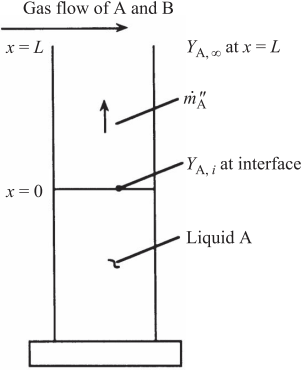
\includegraphics[width=.3\textwidth]{img/stefan.png}
% \end{figure}

我们考虑液体A在玻璃圆通内保持一个固定的高度,假设B在A中不可溶解,由此圆柱中存在着一个B的滞止层。对于这个问题,A的质量通量为:

{\tiny\begin{equation}
    \dot{m}''_A = \frac{\rho \mathcal{D}_\mathrm{AB}}{L}\ln\left(\frac{1-Y_{A,\infty}}{1-Y_{A,i}}\right)
\end{equation}
}
推导过程如下:
{\scriptsize\color{gray}

由于B的量通量为0,基于菲克定律式~\ref{equ:fick_law_1d},我们可以写出
\[
    \dot{m}_A'' = Y_A\dot{m}_A'' - \rho \mathcal{D}_\mathrm{AB}\frac{\dd Y_A}{\dd x}
\]对之整理并分离变量:
\[
    -{\frac{\dot{m}_{\mathrm{A}}^{\prime\prime}}{\rho D_{\mathrm{AB}}}}\mathrm{d}x={\frac{\mathrm{d}Y_{\mathrm{A}}}{1-Y_{\mathrm{A}}}}.
\]
积分解得:
\[
    -{\frac{\bar{m}_{\mathrm{A}}^{\prime\prime}}{\rho D_{\mathrm{AB}}}}\,x=-\ln[1-Y_{\mathrm{A}}]+C,
\]结合已知边界条件,\(Y_A(x=0)=Y_{A,i}, Y_A(x=L)=Y_{A,\infty}\)。}

就可以写出质量分数的计算公式:

\begin{equation}
    Y_A(x) = 1 - (1-Y_{A,i})\exp\left(\frac{\dot{m}_A'' x}{\rho\mathcal{D}_\mathrm{AB}}\right)
\end{equation}

\subsubsection{液-气界面的边界条件}

不难写出\(\chi_{A,i} = P_\mathrm{sat}/P\),由此可以确定质量分数应该为:
\begin{equation}
    Y_{A,i} = \frac{P_\mathrm{sat}(T_\mathrm{liq, i})}{P}\frac{\mathrm{MW}}{\mathrm{MW}_\mathrm{mix, i}}
\end{equation}

认为液-气界面上维持温度的连续性,那么:
\[
    T_\mathrm{liq,i}(x=0^-) = T_\mathrm{vap, i}(x=0^+) = T(0)
\]


\subsubsection{液滴蒸发}

\textbf{假设}:
{\scriptsize
    \begin{enumerate}
        \item 蒸发过程是准稳态的。
        \item 液滴的温度均一,进而假设温度为低于液体的沸点的某一定值。
        \item 液滴表面蒸气的质量分数由液滴温度下的液体-蒸气平衡确定。
        \item 假设所有的热物理参数——特别是\(\rho\mathcal{D}\)——是常数。
    \end{enumerate}
}

\textbf{蒸发速率}:

从某种意义上说,这里的液滴蒸发问题其实就是一个加强版的球状的斯蒂芬流。定义\textbf{传质数}\(B_Y\)为:
\begin{equation}
    B_Y = \frac{Y_{A,s}-Y_{A,\infty}}{1 - Y_{A,s}}
\end{equation}
蒸发速率可以被写作:
\begin{equation}\label{equ:evo_rate}
    \dot{m}_A''' = {4\pi r_s \rho \mathcal{D}_\mathrm{AB}}\ln({1+B_Y})
\end{equation}

具体的推倒过程如下所示:

{
    \scriptsize\color{gray}
    首先,液滴的蒸发速率可以被写作
    \[
        \dot{m}(r) = 4\pi r^2 \dot{m}''
    \]
    将之带入到菲克定律~\ref{equ:fick_law_1d}的表达式中,并且认为另一组份滞止,可以得到:
    \[
        \dot{m}_A'' = Y_A\dot{m}_A'' - \rho\mathcal{D}_\mathrm{AB}\frac{\dd Y_A}{\dd r}
    \]
    代入蒸发速率的表达式,并且整理,可以得到:
    \[
        \dot{m}=-4\pi r^2 \frac{\rho \mathcal{D}_\mathrm{AB}}{1-Y_A}\frac{\dd Y_A}{\dd r}
    \]
    首先代入液滴表面的边界条件\(Y_A(r=r_s)=Y_{A,s}\),可以得到:
    \[
        Y_{\mathrm{A}}(r)=1-{\frac{(1-Y_{\mathrm{A,s}})\exp[-\dot{m}/(4\pi\rho \mathcal{D}_{\mathrm{AB}}r)]}{\exp[-\dot{m}/(4\pi\rho \mathcal{D}_{\mathrm{AB}}r_{s})]}}.
    \]
    再代入\(r\to\infty\)时,\(Y_A=Y_{A,\infty}\),可以解得蒸发速率\(\dot{m}\)的最终结果。
}

\textbf{液滴质量守恒}:

显然,液滴质量和蒸发速率之间的关系是:

\begin{equation}
    \frac{\dd m_d}{\dd t}=-\dot{m}
\end{equation}
液滴的质量可以写作:
\begin{equation}
    m_d = \rho_l V = \rho_l \pi D^3/6
\end{equation}
将这两个式子代入到液滴蒸发速率的公式中(式~\ref{equ:evo_rate}),化简唯粉整理,可以得到:
\begin{equation}
    \frac{\mathrm{d}D}{\mathrm{d}t}=-\frac{4\rho \mathcal{D}_\mathrm{AB}}{\rho_{i}D}\mathrm{ln}(1+B_{Y}).
\end{equation}
或者是:
\begin{equation}
    {\frac{\mathrm{d}D^{2}}{\mathrm{d}t}}=-{\frac{8\rho \mathcal{D}_{\mathrm{AB}}}{\rho_{l}}}\ln(1+B_{Y}).
\end{equation}

我们将等式的右边定义为\textbf{蒸发常数}:
\begin{equation}
    K = {\frac{8\rho \mathcal{D}_{\mathrm{AB}}}{\rho_{l}}}\ln(1+B_{Y})
\end{equation}

由此可以得到\(D\)随时间\(t\)的关系式:
\begin{equation}
    D^2(t)=D_0^2 - Kt
\end{equation}
这就是\textbf{\(D^2\)定律}。

\begin{figure}[H]
    \centering
    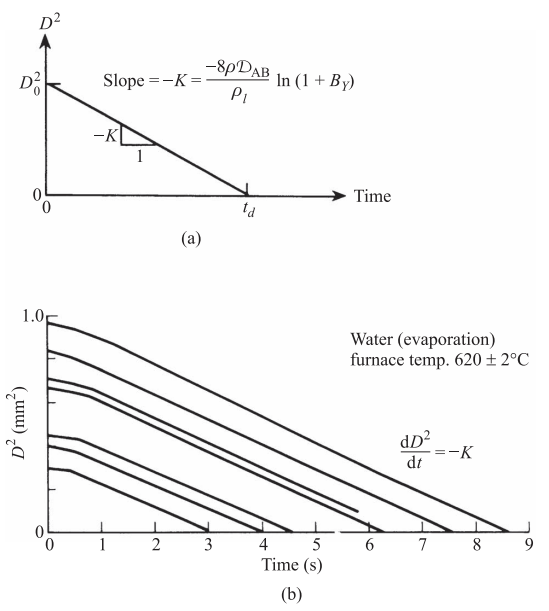
\includegraphics[width=.3\textwidth]{img/d2.png}
\end{figure}

\section{化学动力学}
\subsection{概述}
\subsection{总包反应与基元反应}
燃料和氧化剂的\textbf{总包反应机理}可以被写作:
\begin{equation}
    \mathrm{F} + a\mathrm{Ox}\leftarrow b\mathrm{Pr}
\end{equation}

反应速率可以被表达为:

\begin{equation}
    {\frac{\mathrm{d}[X_{F}]}{\mathrm{d}t}}=-k_{G}(T)[X_{F}]^{n}[X_{O x}]^{m},
\end{equation}其中\(k_G\)为\textbf{总包反应速率常数},\(n\), \(m\)为\textbf{反应级数}。这个式子只在特定的温度和压力范围适用,并且与用于确定反应速率参数的实验装置有关。为了描述一个总体反应所需要的一组基元反应称为\textbf{反应机理}.

\textbf{基团}或\textbf{自由基}是指具有反应性的分子或原子,拥有不成对的电子。

\subsection{基元反应速率}
\subsubsection{双分子反应和碰撞理论}
大部分的基元反应是\textbf{双分子反应}:

\begin{equation}
    \mathrm{A}+\mathrm{B}\rightarrow \mathrm{C} + \mathrm{D}
\end{equation}

反应速率可以写作:
\begin{equation}
    {\frac{\mathrm{d}[{A}]}{\mathrm{d}t}}=-k_{\mathrm{bimolec}}[{A}][{B}].
\end{equation}
如果研究问题的温度范围不是很大,双分子反应速率常数可以用经验的阿累尼乌斯形式(Arrheniusform)来表示,即:
\begin{equation}
    k(T) = A\exp(-E_A/R_u T)
\end{equation}这里的\(A\)是\textbf{指前因子}或\textbf{频率因子}。严格来说它与\(T^{1/2}\)相关。

也有写作:
\begin{equation}
    k(T)=A T^{b}\exp(-E_{A}/R_{u}T),
\end{equation}

\subsubsection{其他基元反应}

\textbf{单分子反应:}
\begin{equation}
    \mathrm{A\rightarrow B}
\end{equation}
或者:
\begin{equation}
    \mathrm{A}\rightarrow \mathrm{B} + \mathrm{C}
\end{equation}

在高压的情况下,这个反应是一阶的,反应速率为:
\begin{equation}
    \frac{\dd \mathrm{A}}{\dd t}=-k_{\mathrm{uni}}[\mathrm{A}]
\end{equation}
在低压时,它还与任意分子的浓度有关,
\begin{equation}
    \frac{\dd[\mathrm{A}]}{\dd t}=-k[\mathrm{A}][\mathrm{M}]
\end{equation}这里的M是任意分子。

\textbf{三分子反应}
\begin{equation}
    \mathrm{A + B + M \rightarrow C + M}
\end{equation}

这里的M同样是任意分子。

\textbf{第三体的作用}:在自由基-自由基反应中,第三体的作用是携带走在形成稳定的组分时释放出来的能量。在碰撞的过程中,新形成的分子的内能传递给第三体 M,成为 M 的动能。没有这一能量的传递,新形成的分子将重新离解为组成它的原子。

\subsection{多步反应机理的反应速率}
\subsubsection{净生成率}
\subsubsection{净生成率的简洁表达式}
对于反应机理,表达式可以写为
\begin{equation}
    \sum_{j=1}^{N}\nu_{j}^{\prime}\,X_{j}\Leftrightarrow\sum_{j=1}^{N}\nu_{j i}^{\prime\prime}\,X_{j}\quad{\mathrm{for}}\quad i=1,2,\dots,L\,,
\end{equation}
净生成率被写作:
\begin{equation}
    \dot{\omega_j}=\sum_{i=1}^L\nu_{ji} q_i\quad{\mathrm{for}}\quad j=1,2,\dots,N\,,
\end{equation}
\begin{equation}
    \nu_{ji} = (\nu_{ji}'' - \nu_{ji}')
\end{equation}
\begin{equation}
    q_i = k_{fi}\Pi_{j=1}^N[X_j]^{\nu_{ji}'} - k_{ri}\Pi_{j=1}^N[X_j]^{\nu_{ji}''}
\end{equation}

\subsubsection{反应速率常数与平衡常数之间的关系}
速率常数不好测,基于热力学测量与计算的平衡常数好测。

\begin{equation}
    \frac{k_f(T)}{k_r(T)} = K_c(T)
\end{equation}

这里的\(K_c\)是基于浓度的平衡常数:
\[K_p = K_c (R_u T/ P^0)^{c+d+\cdots-a-b-\cdots}=K_c (R_u T/ P^0)^{\sum \nu''-\sum \nu'}\]

实际操作中,测定好测的正反应速率常数,然后推算出逆反应的速率常数。

\subsubsection{稳态近似}
在燃烧过程所涉及的许多化学反应系统中,会形成许多高反应性的中间产物,即自由基。针对这类中间产物或自由基,采用稳态近似,就可以大大减少对这些系统的分析工作。从物理上讲,这些自由基的浓度在一个迅速的初始增长后,其消耗与形成的速率就很快趋近,即生成和消耗速率是相等的。

\subsubsection{单分子反应机理}

考虑第三体的作用,产物的生成速率应当等于激活的A分子浓度成一阶反应的速率常数:

\begin{equation}
    \frac{\dd[\mathrm{products}]}{\dd t}=k_\mathrm{uni}[\mathrm{A^*}]
\end{equation}

利用稳态近似,认为激活的A分子浓度不变,可以将A\(^*\)的净生成率表达成为:

\begin{equation}
    {\frac{\mathrm{d}[\mathrm{A}^{*}]}{\mathrm{d}t}}=k_{e}[\mathrm{A}][\mathrm{M}]-k_\mathrm{d e}[\mathrm{A}^{*}][\mathrm{M}]-k_{\mathrm{uni}}[\mathrm{A}^{*}].
\end{equation}

经过层层推导可以得到如下的结论:

\begin{equation}\label{equ:unimol_react}
    -\frac{\dd[\mathrm{A}]}{\dd t}=\frac{\dd[\mathrm{products}]}{\dd t} = k_\mathrm{app}[\mathrm{A}]
\end{equation}其中\(k_\mathrm{app}\)被定义为单分子反应的\textbf{表观速率常数},计算公式为:

\begin{equation}
    k_\mathrm{app}=\frac{k_e[\mathrm{M}]}{(k_\mathrm{de}/k_\mathrm{uni})[\mathrm{M}]+1}
\end{equation}

\subsubsection{链式反应和链式分支反应}

对于总包反应

\begin{equation}
    \mathrm{A_2+B_2}\rightarrow 2\mathrm{AB}
\end{equation}

\textbf{链的激发反应}为:
\begin{equation}
    \mathrm{A_2+M}\overset{k_1}{\longrightarrow} \mathrm{A+A+M}
\end{equation}
\textbf{链的传播反应}为:
\begin{eqnarray}
    \mathrm{A+B_2\overset{k_2}{\longrightarrow}AB + B}\\
    \mathrm{B+A_2\overset{k_3}{\longrightarrow}AB + A}
\end{eqnarray}
\textbf{链的终止反应}为:
\begin{equation}
    \mathrm{A+B+M\overset{k_4}{\longrightarrow}AB+M}
\end{equation}

分析过程太复杂,可以看书100页。几个结论:
\begin{equation}
    [\mathrm{A}]\approx{\frac{[\mathrm{A}_{2}]}{[\mathrm{B}_{2}]^{1/2}}}\left({\frac{k_{1}k_{3}}{k_{2}k_{4}}}\right)^{1/2}
\end{equation}

\begin{equation}
    \frac{\mathrm{d}[{\mathrm{B}}_{2}]}{\mathrm{d}t}\approx-[{\mathrm{A}}_{2}][{\mathrm{B}}_{2}]^{1/2}\left(\frac{k_{1}k_{2}k_{3}}{k_{4}}\right)^{1/2}.
\end{equation}
\begin{enumerate}
    \item 链的激发反应速率越大,链的中断反应速率常数越小,自由基的浓度也越大。
    \item 增大链的传递反应速率常数,会增大\([\mathrm{B_2}]\)的消耗速率。
    \item 链的传递反应速率常数对自由基的浓度影响不大。因为由于其速率常数具有相同的量级且以一个比值的方式出现。
\end{enumerate}

压力足够高时,由于假设的\(4k_2 k_3[B_2]/(k_1 k_4[M]^2)\gg 1\)不再成立,上面的结论也不再可靠。

\textbf{链式分支反应}是指:\textit{消耗一个}自由基而\textit{形成两个}自由基组分的反应。链式分支反应对具有自传播特性的火焰起主导作用,这也是燃烧化学中最基本的特征。

\textbf{化学时间尺度}

\begin{enumerate}
    \item 单分子反应
    我们对单分子反应速率的表达式\ref{equ:unimol_react}进行积分,得到:
    \begin{equation}
        [\mathrm{A}](t)=[\mathrm{A}]_{0}\exp(-k_{\mathrm{app}}t)
    \end{equation}其中[A]\(_0\)为组份A的初始浓度. 如果用RC电路定义特征时间的方法,我们可以得到\textbf{化学时间尺度}的表达式:
    \begin{equation}
        \tau_\mathrm{chem} = 1/k_\mathrm{app}
    \end{equation}

    \item 双分子反应
    对于如下的反应
    \[
        \mathrm{A+B\rightarrow C+D}
    \]
    它的速率表达式为:
    \begin{equation}
        \frac{\dd [\mathrm{A}]}{\dd t}=-k_\mathrm{bimolec}\mathrm{[A][B]}
    \end{equation}
    A和B的浓度变化可以通过化学当量关系来联系, 经过推导之后最后得到结论:
    \begin{equation}
        \tau_{\mathrm{chem}}={\frac{\mathrm{ln}[e+(1-e)\mathrm{([A]_{0}/[B]_{0})}]}{([\mathrm{B}]_{0}-\mathrm{[A]}_{0})k_{\mathrm{bimodec}}}},
    \end{equation}其中\(e=2.718\).

    如果其中反应物浓度要比另一种大得多,比如B很大,那么上面的式子可以简化为:
    \begin{equation}
        \tau_\mathrm{chem}=\frac{1}{[\mathrm{B}]_0 k_\mathrm{bimolec}}
    \end{equation}

    \item 三分子反应
    \[\mathrm{A+B+M\rightarrow C + M}\]
    如果我们认为第三体浓度[M]是一个常数,我们可以得到和双分子反应类似的结论:
    \begin{equation}
        {\frac{\mathrm{d}[\mathrm{A}]}{\mathrm{d}t}}=(-k_{\mathrm{ter}}[\mathrm{M}])[\mathrm{A}][\mathrm{B}].
    \end{equation}

    \begin{equation}
        \tau_{\mathrm{chem}}={\frac{\mathrm{ln}[e+(1-e)([\mathrm{A}]_{0}/[\mathrm{B}]_{0})]}{([\mathrm{B}]_{0}-[\mathrm{A}]_{0})k_{\mathrm{te}}[\mathrm{M}]}},
    \end{equation}


    类似地, 如果B的浓度远远大于A, 那么:
    \begin{equation}
        \tau_{\mathrm{chem}}=\frac{1}{[{\rm B}]_{0}[{\rm M}]k_{\mathrm{ter}}}.
    \end{equation}
\end{enumerate}

\subsubsection{部分平衡}
将\textit{快速反应}视作\textit{平衡态}处理可以简化化学动力学机理,从而无须写出所涉及自由基的速率方程。这种处理方法叫作部分\textbf{平衡近似}。

\section{一些重要的化学机理}

\subsection{概述}
\subsection{\(\mathrm{H_2-O_2}\)系统}

\begin{multicols}{2}
{\fontsize{4}{1}\selectfont
初始激发反应(第一个为高温, 第二个为其他温度):
\begin{eqnarray}
    \mathrm{H_2+M}&\to&\mathrm{H+H+M}\\
    \mathrm{H_2+O_2}&\to&\mathrm{HO_2+H}\label{equ:activate}
\end{eqnarray}
包含有自由基 0,H 和 OH 的链式反应是:
\begin{eqnarray}
    \mathrm{H+O_2}&\to& \mathrm{O+OH}\label{equ:chain1}\\
    \mathrm{O + H_2}&\to& \mathrm{H + OH}\\
    \mathrm{H_2+OH}&\to& \mathrm{H_2O+H}\\
    \mathrm{O+H_2O}&\to& \mathrm{OH+OH}\label{equ:chain4}
\end{eqnarray}
包含自由基 O,H 和 OH 自由基的链的中断反应是三分子化合反应
\begin{eqnarray}
    \mathrm{H+H+M}&\to&\mathrm{H_2+M}\\
    \mathrm{O+O+M}&\to& \mathrm{O_2+M}\\
    \mathrm{H+O+M}&\to& \mathrm{OH + M}\\
    \mathrm{H + OH + M} &\to& \mathrm{H_2O + M}
\end{eqnarray}

过氧羟基和双氧水的反应也很重要, 当这个反应变得活跃是:
\begin{equation}\label{equ:HO2}
    \mathrm{H+O_2+M}\to \mathrm{HO_2 +M}
\end{equation}

下列反应和第二个反应的逆反应开始起作用:
\begin{eqnarray}
    \mathrm{HO_2+H} &\to& \mathrm{OH+OH} \\
    \mathrm{HO_2+H} &\to& \mathrm{H_2O+O} \\
    \mathrm{HO_2+O} &\to& \mathrm{O_2+OH} \\
    \mathrm{HO_2+HO_2} &\to& \mathrm{H_2O_2+O_2} \\
    \mathrm{HO_2+H_2} &\to& \mathrm{H_2O_2+H} \label{equ:H2O2}\\
    \mathrm{H_2O_2+OH} &\to& \mathrm{H_2O+HO_2} \\
    \mathrm{H_2O_2+H} &\to& \mathrm{H_2O+OH} \\
    \mathrm{H_2O_2+H} &\to& \mathrm{HO_2+H_2} \\
    \mathrm{H_2O_2+M} &\to& \mathrm{OH+OH+M}
\end{eqnarray}
}
\end{multicols}
关于书本图5.1爆照极限的分析(500$^\circ$C 这一条线来讨论爆炸行为):
\begin{enumerate}
    \item 小于1.5 mmHg, 无爆炸,这是因为~\ref{equ:activate}激发的步骤和后面的链式反应~\ref{equ:chain1}-\ref{equ:chain4}所产生的自由基被避免反应所消耗而中断.
    \item 高于1.5 mmHg爆炸就会发生是因为\ref{equ:chain1}-\ref{equ:chain4}所产生的自由基超过了壁面的消耗速度(压力增加导致自由基的浓度呈线性增加,相应的反应速率呈几何增加。).
    \item 高于50 mmHg时, 混合物又停止了爆炸的特性, 这是由于链式分支反应~\ref{equ:chain1}和低温下显著的链中断反应~\ref{equ:HO2}之间产生了竞争. 过氧羟基相对不活跃, \ref{equ:HO2}可以被看作是链中断反应, 产生的自由基扩散到了壁面被消耗.
    \item 高于3000 mmHg时, \ref{equ:H2O2}加入到了链式分支反应中,引起了双氧水的链式反应过程.
\end{enumerate}

\subsection{一氧化碳的氧化}

不含水时,一氧化碳的氧化非常缓慢, 少量水的影响非常大, 因为羟基很重要.

\begin{eqnarray}
    \mathrm{CO+O_2} &\to& \mathrm{CO_2+O} \\
    \mathrm{O + H_2O} &\to& \mathrm{OH + OH} \\
    \mathrm{CO + OH} &\to& \mathrm{CO_2 + H} \label{equ:CO_burn}\\
    \mathrm{H + O_2} &\to& \mathrm{OH + O}
\end{eqnarray}

第一个反应激发链式反应, CO的实际氧化通过第三个反应完成.

如果催化剂为氢气, 那么还会包括氢气和氧原子, 氢气和羟基的反应. 实质上, 在有氢的情况下,为了描述CO的氧化, 需要包含上面提到的所有氢氧反应. 此外, 在过氧羟基存在的基础上, 还需要包括它氧化CO生成水和二氧化碳的反应.

\subsection{碳氢化合物的氧化}
碳氢化合物的燃烧可以简单地分为两步:第一步包括燃料断裂生成一氧化碳;第二步是一氧化碳最终氧化成为二氧化碳。

\subsubsection{链烷烃概况}

链烷烃, aka. 石蜡类物质, 化学分子式\(\mathrm{C_n H_{2n+2}}\). 这里先讨论\(n>2\)的情况.
\begin{enumerate}
    \item  燃料分子受到O和H原子的撞击而分解,先分解成烯烃和氢。在有氧存在的情况
下,氢就氧化成水。
    \item 不饱和烯烃进一步氧化成为CO和\(\mathrm{H_2}\), 所有的\(\mathrm{H_2}\)都转化为水.
    \item CO通过~\ref{equ:CO_burn}燃尽, 热量主要在这一步释放.
\end{enumerate}

具体展开如下:
\begin{enumerate}
    \item 薄弱的C-C键先于C-H键断裂, 产生碳氢自由基.
    \item \textbf{脱氢}: 碳氢自由基进一步分解, 产生烯烃和氢原子.
    \item 上一步中的氢原子进一步产生新的自由基(羟基和氧原子).
    \item 自由基的累计开始了新的燃料分子被撞击的过程.
    \item 生成的碳氢自由基进一步脱氢(基于\(\beta\)剪刀原则展开).
    \item 烯烃由O原子撞击产生氧化, 生成甲酸基(HCO)和甲醛(H\(_2\)CO).
    \item 甲基, 甲醛, 亚甲基氧化,
    \item 按含湿的 CO 机理进行的一氧化碳的氧化.
\end{enumerate}

\textbf{\(\beta\)剪刀原则:} 断裂C-C或C-H键将是离开自由基位置的一个键(离开不成对电子的一个位置). 这是因为在自由基位置处的不成对电子加强了相邻的键, 导致了从这一位置向外移动了一个位置.

\subsubsection{总包和准总包机理}

一步总包:
\begin{equation}
    \mathrm{C}_x \mathrm{H}_y + (x+y/4)\mathrm{O_2} \to x\mathrm{CO_2} + y/2\mathrm{H_2O}
\end{equation}

四步反应模拟丙烷的氧化:
\begin{enumerate}
    \item \(\mathrm{C}_n \mathrm{H}_{2n+2} \to (n/2) \mathrm{C}_2 \mathrm{H}_4 + \mathrm{H}_2\)
    \item \(\mathrm{C}_2\mathrm{H}_4 + \mathrm{O}_2 \to 2\mathrm{CO} + 2 \mathrm{H}_2\)
    \item \(\mathrm{CO+\frac{1}{2}O_2\to CO_2}\)
    \item \(\mathrm{H_2 + \frac{1}{2}O_2\to H_2O}\)
\end{enumerate}

\subsubsection{实际燃料及其替代物}

\subsection{甲烷燃烧}
\subsubsection{复杂机理}
\subsubsection{高温反应途径分析}
\begin{enumerate}
    \item 主线从OH, O和H撞击CH\(_4\)产生甲基自由基开始;
    \item 甲基自由基和氧原子产生甲醛;
    \item 甲醛由OH, H和O撞击形成甲酸基;
    \item 甲酸基通过三个反应形成CO;
    \item CO变成CO\(_2\).
\end{enumerate}

除了这一途径, 还有一些其他途径:
\begin{enumerate}
    \item 甲基形成两种可能电子结构的亚甲基
    \item 甲基形成甲醇, 然后变成甲醛.
\end{enumerate}
\subsubsection{低温反应途径分析}
几个有趣现象:
\begin{enumerate}
    \item 存在较强的甲基重新变成甲烷的现象;
    \item 通过甲醇, 出现了从甲基到甲醛的新途径;
    \item 甲基变成了乙烷, 乙烷变成乙烯和乙炔然后变成一氧化碳和亚甲基(出现比初始弹琴化合物高的碳氢化合物是低温氧化过程的一个共同特点).
\end{enumerate}

\subsection{氮氧化物的形成}

热力型机理在高温燃烧中起支配作用,当量比可以在很
宽的范围内变化。而费尼莫机理在富燃料燃烧中特别重要。NO-中间体机理在很贫的燃
料和低温燃烧过程中对 NO 的产生有很重要的作用。NNH 机理相对上面提到的机理是新
提出的。针对预混火焰加和扩散火焰[27胸多方面的研究发展了前三种机理,而对于在射流
混合反应器中贫燃料预混燃烧的研究,对全部四种机理作出了相应贡献[29]。要获得比在本
节中提供的在燃烧过程中氮氧化物形成与控制的化学的更详细资料,读者可以参考 Dagaut
等L3o]、Dean 和 Bozzelli 及 Miller 和 Bowman位等的综述文章。进一步的信息和参考文
献参见第 15 章。

\begin{enumerate}
    \item \textbf{热力型机理}在高温燃烧中起支配作用,当量比可以在很宽的范围内变化。
    \item \textbf{费尼莫机理}在富燃料燃烧中特别重要。
    \item \textbf{N\(_2\)O-中间体机理}在很贫的燃料和低温燃烧过程中对 NO 的产生有很重要的作用。
    \item \textbf{NNH机理}相对上面提到的机理是新提出的。
\end{enumerate}

\textbf{热力型机理, Zeldovich}:
\begin{eqnarray}
    \mathrm{O+N_2} &\leftrightarrow& \mathrm{NO + N}\\
    \mathrm{N+O_2} &\leftrightarrow& \mathrm{NO + O}\\
    \mathrm{N+OH} &\leftrightarrow& \mathrm{NO + H}
\end{eqnarray}
按理说这个反应会通过氧气, 羟基和氧原子与燃烧发生耦合. 但是由于一般只有在燃烧完全后, NO的形成才会明显, 所以他们一般不耦合. 在此情况下, 如果认为
\begin{enumerate}
    \item 反应尺度够长\(\to\)氮气, 氧气, 氧原子和羟基浓度处于平衡值;
    \item NO浓度远小于平衡值\(\to\)逆反应忽略
\end{enumerate}

那么NO的生成就只和氧原子和氮气相关.

当然在火焰区, 时间尺度小, 平衡假设不成立. 此时O处于超平衡浓度, 大大加快了NO的形成速率(有时归结为快速型NO机理, 考虑历史, 快速限定为费尼莫尔机理).
由于活化能大, 所以高温下此机理才重要. 又由于时间尺度小于燃料氧化的时间尺度, 因此NO往往在火焰后的气体中产生.

\textbf{N\(_2\)O-中间体机理}
在贫燃料(\(\phi<0.8\))和低温的条件下, N\(_2\)O-中间体机理很重要 (燃气轮机制造商):

\begin{eqnarray}
    \mathrm{O + N_2 + M} &\leftrightarrow& \mathrm{N_2O + M}\\
    \mathrm{H + N_2O} &\leftrightarrow& \mathrm{NO + NH}\\
    \mathrm{O + N_2O} &\leftrightarrow& \mathrm{NO + NO}
\end{eqnarray}


\textbf{费尼莫儿机理/快速型NO}
得名原因: 费尼莫尔最早发现 NO 在层流预混火焰的火焰区域中快速地产生,且是在热力型 NO 形成之前就已形成。
\begin{eqnarray}
    \mathrm{CH + H_2} &\leftrightarrow& \mathrm{HCN + N}\\
    \mathrm{C + N_2} &\leftrightarrow& \mathrm{CN + N}
\end{eqnarray}

在当量比小于1.2时, HCN由下面的方法产生NO:

\begin{eqnarray}
    \mathrm{HCN + O} &\leftrightarrow& \mathrm{NCO + H} \\
    \mathrm{NCO + H} &\leftrightarrow& \mathrm{HN + CO} \\
    \mathrm{NH + H} &\leftrightarrow& \mathrm{N + H_2} \\
    \mathrm{N + OH} &\leftrightarrow& \mathrm{NO + H}
\end{eqnarray}

当量比大于1.2时, 会比较复杂.

如果上面的反应不快速的时候, NO会形成HCN, 然后反应就倒过来了, 氧化变成了还原.

\textbf{NNH机理}: 

对氢的燃烧, 大碳氢比燃料的燃烧很重要:

\begin{eqnarray}
    \mathrm{N_2 + H} &\leftrightarrow& \mathrm{NNH}\\
    \mathrm{NNH + O} &\leftrightarrow& \mathrm{NO + NH}
\end{eqnarray}

\textbf{燃料氮}:

燃料中含有的氮,这些氮形成的NO是燃料氮,也是一个重要的途径。

\end{multicols}


\end{document}